\documentclass[conference]{IEEEtran}
\IEEEoverridecommandlockouts
% The preceding line is only needed to identify funding in the first footnote. If that is unneeded, please comment it out.
\usepackage{cite}
\usepackage{amsmath,amssymb,amsfonts}
\usepackage{algorithm}
\usepackage{algorithmic}
\usepackage{graphicx}
\usepackage{textcomp}
\usepackage{xcolor}
\usepackage{tabularx}
\usepackage{url}
\usepackage{array}
\renewcommand{\IEEEkeywordsname}{Keywords}
\usepackage{listings}
\def\BibTeX{{\rm B\kern-.05em{\sc i\kern-.025em b}\kern-.08em
    T\kern-.1667em\lower.7ex\hbox{E}\kern-.125emX}}
\newcolumntype{Y}{>{\raggedright\arraybackslash}X}
\begin{document}

\title{\textbf{Artificial Intelligence for EDA Tool Automation: A Review of AI-Driven VLSI Design Workloads}}



\author{
\IEEEauthorblockN{
\makebox[\linewidth][c]{%
\makebox[0.45\textwidth][c]{\textbf{Pranav Jois}}%
\hspace{0.05\textwidth}%
\makebox[0.45\textwidth][c]{\textbf{Rohit L}}%
}}
\IEEEauthorblockA{
\begin{minipage}[t]{0.45\textwidth}
\centering
\textit{Roll No. 231EC237}\\
\textit{Mobile No. 9686326473}\\
\textit{pranavjois.231ec237@nitk.edu.in}\\
\textit{Electronics \& Communication Engineering Department}\\
\textit{National Institute of Technology Karnataka, Surathkal}
\end{minipage}
\hspace{0.05\textwidth}
\begin{minipage}[t]{0.45\textwidth}
\centering
\textit{Roll No. 231EC248}\\
\textit{Mobile No. 9482962815}\\
\textit{rohitlalu.231ec248@nitk.edu.in}\\
\textit{Electronics \& Communication Engineering Department}\\
\textit{National Institute of Technology Karnataka, Surathkal}
\end{minipage}
}\\[1em]

\IEEEauthorblockN{
\makebox[\linewidth][c]{%
\textbf{Prateek Goel}
}}

\IEEEauthorblockA{
\begin{minipage}[t]{0.7\textwidth}
\centering
\textit{Roll No. 231EC142}\\
\textit{Mobile No. 9620204015}\\
\textit{prateekgoel.231ec142@nitk.edu.in}\\
\textit{Electronics \& Communication Engineering Department}\\
\textit{National Institute of Technology Karnataka, Surathkal}
\end{minipage}
}
}

\maketitle



\begin{abstract}
The growing complexity of modern VLSI systems has made Electronic Design Automation (EDA) tools essential for hardware development. However, existing workflows still require multiple tools, repetitive scripting, and extensive design-space exploration. Recent advances in artificial intelligence (AI), machine learning (ML), and large language models (LLMs) offer ways to automate these tasks. This paper reviews and compares fourteen studies on AI-driven EDA, covering ML-based prediction and optimisation, graph neural networks (GNNs), RTL generation, domain-adapted LLMs, and autonomous EDA agents. The studies are classified by AI technique, design stage, and a five-level automation scale introduced in this paper. Software engineering principles, including modularity, interoperability, testing, and reproducibility, guide the analysis of research gaps and the identification of future directions. The paper also presents a methodology for measuring how evaluation choices affect RTL generation pass@1, validated first on synthetic models with known behaviour and then applied to two small open models on a 30-problem subset of VerilogEval, where the sampling seed is found to move the reported pass@1 far more than the prompt wording, code-extraction rule, or module-naming convention combined---enough that a single run can misorder two models of visibly different ability. The review highlights fragmented research, inconsistent evaluation practices, and the continued need for reliable verification of AI-generated designs.
\end{abstract}
\vspace{0.5cm}
\begin{IEEEkeywords}
Artificial Intelligence, VLSI, Machine Learning, Large Language Models, Electronic Design Automation, RTL Generation, Software Engineering
\end{IEEEkeywords}


\section{Introduction}
The complexity of integrated circuits has made modern VLSI design increasingly dependent on Electronic Design Automation (EDA) tools. Contemporary digital systems integrate processors, memories, communication interfaces, accelerators, and specialised hardware blocks containing millions or billions of transistors. Designing and validating such systems manually is impractical. EDA tools, therefore, automate a large portion of the design process, including hardware description, logic synthesis, placement, routing, timing analysis, power analysis, verification, and physical implementation.\\

\noindent Despite the capabilities of modern EDA tools, the complete design process remains complex and iterative. A typical digital design requires several specialised tools, each with its own input formats, scripting interfaces, constraints, libraries, and report formats. Engineers must configure individual tools, execute scripts, analyse reports, modify design parameters, and repeat the process. Design space exploration further increases effort because many combinations of architectural, synthesis, and physical design parameters may need to be evaluated before acceptable power, performance, and area (PPA) are achieved.\\

\noindent Artificial intelligence has increasingly been investigated as a means of reducing this burden. Machine learning (ML) techniques have been applied to prediction, optimisation, design space exploration, and other EDA problems. Huang et al.\ survey ML applications across the EDA hierarchy and show how learning-based methods have been applied at multiple stages of chip design \cite{P1_Huang2021}. Chen et al.\ examine ML methodologies for advanced IC design and identify the large design space and growing complexity of modern ICs as the central motivations for AI based methods \cite{P2_Chen2023}. Concrete results include deep reinforcement learning for chip floorplanning, which produced floorplans comparable or superior to human designs in power, performance, and area within hours \cite{P8_Mirhoseini2021}, and ML models that estimate PPA directly from RTL without running synthesis \cite{P10_Fang2023}.\\

\noindent Graph neural networks (GNNs) have attracted attention because circuits naturally possess graph structure. Gates, cells, nets, and their connectivity can be represented as graphs, allowing graph-based models to learn structural information. S{\'a}nchez et al.\ review the relationship between GNNs and EDA and classify existing work according to circuit representations, tasks, and model types \cite{P3_Snchez2023}.\\

\noindent More recently, large language models (LLMs) have introduced a different form of AI assisted hardware design. Rather than limiting AI to numerical prediction or optimisation, LLMs can process natural language specifications and generate hardware description language (HDL) code, scripts, documentation, and other design artefacts. Fine tuned open models for Verilog generation \cite{P11_Thakur2024,P4_Liu2025}, benchmarks for assessing them \cite{P12_Liu2023,P15_Pinckney2025}, and conversational co-design studies \cite{P13_Blocklove2023} have established RTL generation as an active research area. The broader experience with LLMs as code generators, where fluent output can mask subtle functional errors, has already prompted careful scrutiny of how these systems are evaluated \cite{10.1007/s10844-025-00968-y}; the same caution applies with greater force to hardware, where a plausible-looking module must still be synthesised and verified. LLM use has also expanded from isolated code generation towards interaction with complete EDA workflows. ChatEDA investigates an LLM-powered autonomous agent that performs task planning, script generation, and execution with EDA tools as executors \cite{P5_Wu2024}, while ChipNeMo studies domain adaptation of LLMs for industrial chip design \cite{P14_Liu2023ChipNeMo}. Recent surveys broaden the analysis of LLMs across EDA, including code generation, verification, knowledge representation, and optimisation \cite{P6_Pan2025,P7_He2025}.\\

\noindent These developments indicate a progression from conventional EDA automation towards AI assisted and increasingly AI-integrated workflows. However, the research is distributed across different EDA stages and AI techniques, and individual studies rarely use common benchmarks or metrics. A structured comparison is therefore useful for understanding which problems have been addressed, which advantages have been demonstrated, and which limitations remain.\\

\noindent This paper presents a survey and comparative analysis of AI-driven EDA automation research. Its objectives and contributions are as follows:
\begin{itemize}
    \item To review the evolution of AI applications in EDA, from ML-based prediction to LLM-based agents.
    \item To classify existing approaches according to the AI technique, the VLSI design stage, and a five-level scale of automation.
    \item To compare the strengths and limitations of the approaches in a single consolidated table.
    \item To identify common research gaps across the existing studies.
    \item To examine how software engineering principles can improve the reliability and maintainability of AI-driven EDA workflows.
    \item To specify a methodology for measuring how much evaluation choices move the reported pass@1 of LLM-generated RTL, and to validate it on synthetic models with known effects.
\end{itemize}

\subsection{Conventional VLSI Design Workflow} \label{B1}

\noindent A conventional digital VLSI design process consists of multiple stages as seen in Fig. \ref{fig_design_flow}. The process generally begins with a system specification, which is converted into an RTL description using languages such as Verilog or SystemVerilog. Functional simulation and verification are then performed to determine whether the RTL satisfies the required behaviour. The RTL stage is particularly consequential because designers define precise behaviour there and make fine-grained decisions that ultimately determine PPA, yet the quality of an RTL design is conventionally assessed only by running the subsequent synthesis steps \cite{P10_Fang2023}.\\

\begin{figure*}[!t]
\centering
\includegraphics[width=0.85\textwidth]{asic_flow.png}
\caption{Conventional digital VLSI design flow.}
\label{fig_design_flow}
\end{figure*}


\noindent After functional verification, logic synthesis converts the RTL into a gate-level representation using a target standard cell library. Physical design subsequently includes floorplanning, placement, clock tree synthesis, and routing. Timing analysis, power analysis, design rule checking (DRC), and layout versus schematic (LVS) verification are performed before final manufacturing data is generated.\\

\noindent The stages are not strictly linear. A timing violation discovered after synthesis or physical implementation may require modifications to the RTL, synthesis constraints, or physical design parameters. Similarly, excessive area or power may trigger another iteration of the flow. The iterative nature of the flow makes automation particularly valuable. However, conventional automation is predominantly based on predefined scripts and tool specific commands. This provides reproducibility but requires significant domain knowledge.

\subsection{Limitations of Traditional Automation} \label{B2}

\noindent \textbf{Tool heterogeneity.} Complete flows may involve simulators, synthesis tools, place and route tools, timing analysis tools, and physical verification tools. These tools often use different command languages, constraint formats, and report formats, so engineers carry the burden of integration.

\noindent \textbf{Expensive design space exploration.} Numerous parameters affect PPA, timing closure, routability, and other objectives. Exhaustive exploration requires many computationally expensive EDA runs, and each run may take hours for large designs. Logic synthesis alone is a combinatorial optimisation problem in which the choice of transformation sequence influences the final netlist quality \cite{P9_Chowdhury2021}.

\noindent \textbf{Static procedures.} Traditional scripts follow predefined procedures. They do not naturally interpret unstructured design requirements or dynamically change the workflow based on information contained in generated reports.

\noindent \textbf{No reuse of experience.} Knowledge from previous design iterations is not automatically reused. Engineers rely on experience to select parameters or recognise patterns in reports, whereas scripts execute predetermined instructions.

\noindent These limitations have motivated research into ML based prediction and optimisation and, more recently, LLM based assistance and automation \cite{P1_Huang2021,P2_Chen2023,P6_Pan2025}.

\subsection{Role of Artificial Intelligence in EDA} \label{B3}

\noindent AI applications in EDA can broadly be grouped into three categories: 
\begin{itemize}
    \item \textbf{Prediction}: An AI model estimates a design property that would otherwise require a computationally expensive EDA operation, such as timing, power, area, routability, or other quality metrics. \\

    \item \textbf{Optimisation}: AI is used to search a large design space and identify promising configurations. ML and reinforcement learning (RL) techniques can guide such searches \cite{P1_Huang2021,P2_Chen2023}. In the RL formulation, a policy interacts with a design environment through states, actions, and rewards derived from quality metrics, and is trained to maximise the expected return.\\
    
    \item \textbf{Generation and interaction}: AI generates RTL, scripts, testbenches, constraints, explanations, or tool commands. LLM based approaches primarily belong to this category, although they can also support optimisation and analysis.\\
\end{itemize}

\noindent These categories are complementary rather than mutually exclusive. A future EDA workflow may use different AI techniques for different tasks rather than relying on a single model for the entire design process.

\subsection{Software Engineering Perspective} \label{B4}

\noindent Since AI driven EDA couples probabilistic models with deterministic tools, the resulting workflow is a software system in its own right. This paper, therefore, evaluates the literature against six software engineering principles: \\\\
\textbf{Modularity} is the decomposition of the workflow into components with well defined responsibilities. \\ \textbf{Abstraction} hides tool specific detail behind stable interfaces. \\
\textbf{Interoperability} is the ability of components to exchange data through standard formats.\\
\textbf{Testing} is the systematic checking of every generated artefact against an independent oracle. 
\\
\textbf{Reproducibility} is the ability to regenerate a result from recorded inputs, versions, and settings. \\
\textbf{Human oversight} is the explicit placement of review and approval points. \\\\
 The remainder of the paper is organised as follows. Section~\ref{sec_litrev} reviews the literature and presents the comparative analysis and identifies research gaps. Section~\ref{sec_method} specifies and validates a methodology for measuring evaluation sensitivity. Section~\ref{sec_conclusion} concludes the discussion.

\section{Literature Review}\label{sec_litrev}

The reviewed research is subdivided into five groups: ML for EDA, GNNs for EDA, LLM assisted RTL generation, domain adapted LLM assistants, LLM surveys, and autonomous EDA agents. The works look similar at first glance, but they separate along one axis that organises the rest of this section: how much of the design task the AI actually performs, from a single prediction to a full tool-driving agent.
\\\\
Each work is classified along three dimensions: the \textbf{AI technique} (ML, GNN, RL, LLM, LLM agent), the \textbf{design stage} (RTL, logic synthesis, physical design, or the whole flow), and the \textbf{degree of automation}. The last dimension reflects who performs the execution and who verifies the result. Five levels are: 
\begin{itemize}
    \item \textbf{L0 (Scripted)}: Fixed scripts execute the flow, the engineer interprets reports and decides.
    \item \textbf{L1 (Advisory)}: A model predicts or ranks, the engineer decides and acts.
    \item \textbf{L2 (Generative)}: A model produces an artefact (RTL, script, placement) and the engineer reviews and verifies it.
    \item \textbf{L3 (Supervised agent)}: A model plans and invokes tools across several steps, the engineer supervises and approves.
    \item \textbf{L4 (Autonomous)}: Closed loop of planning, execution, and verification without a human in the loop.
\end{itemize}


\subsection{Machine Learning for EDA} \label{L1}

\noindent ML based EDA research predates the recent growth of LLMs. Huang et al.\ survey ML techniques across the EDA hierarchy \cite{P1_Huang2021}. Their review shows that ML can learn relationships between design characteristics and outcomes, which makes it useful both for predicting results and for guiding optimisation. A major advantage is the ability to approximate expensive evaluations. If a model accurately predicts a design metric, designers can reduce the number of full EDA executions required during exploration, thereby allowing ML to serve as a surrogate for selected operations.\\

\noindent Chen et al.\ analyse ML methods from both the IC design problem perspective and the ML method perspective \cite{P2_Chen2023}. Their analysis emphasises the large and complex design space of advanced IC design. Different learning methods suit different problems, and the usefulness of an ML model depends strongly on the quality and relevance of its training data.\\

\noindent \textbf{Prediction at RTL:} MasterRTL is a representative primary study of early prediction \cite{P10_Fang2023}. Addresses the problem that assessing the quality of an RTL design typically requires time consuming synthesis, which impedes optimization at the early RTL stage. The framework converts HDL code into a bit-level representation, the simple operator graph (SOG), built only from single-bit simple operators, so that different design types and styles are unified and the representation resembles the target gate-level netlist. Separate ML models then estimate timing, power, and area, and the timing model explicitly captures the critical path and the delay between register pairs. The authors also extend the framework to post-placement PPA. MasterRTL illustrates both the promise and the dependence of surrogate models on data: their value depends on how well the training designs cover those encountered later.\\

\noindent \textbf{Data for ML-guided synthesis:} OpenABC-D addresses the absence of standard datasets for ML guided logic synthesis \cite{P9_Chowdhury2021}. It was produced by synthesising open-source hardware designs with random synthesis recipes using an open-source synthesis tool, yielding And-Inverter Graphs (AIGs) with labels such as node count, longest path, area, and delay, and defining learning problems such as predicting the quality of a recipe's result. Datasets of this kind are a prerequisite for comparable evaluation. Still, a dataset generated using a single open-source tool and a limited number of designs does not, by itself, represent industrial flows.\\

\noindent \textbf{Optimisation in Physical Design:} Mirhoseini et al.\ pose chip floorplanning as an RL problem and use an edge-based graph convolutional network to learn transferable representations of the chip \cite{P8_Mirhoseini2021}. In under six hours, the method generates floorplans reported to be superior to or comparable to those of human designers in power, performance, and area, and it was used to design the next generation of Google's AI accelerators. This work is the strongest example in the surveyed set of AI optimisation that has reached production use. Its scope, however, is a single stage, floorplanning, and the approach inherits the computational cost and data requirements of RL training.\\

\noindent Taken together, the literature suggests that ML is particularly valuable for specialised EDA tasks. Still, the resulting models are designed for specific problems rather than for end-to-end automation, and each depends on labelled data produced by the very tools it is meant to relieve.

\subsection{Graph Neural Networks in EDA}\label{L2}

\noindent Circuit designs have an inherent graph structure. Components can be represented as nodes, and electrical or logical connections as edges, making GNNs particularly relevant to circuit analysis. \\

\noindent S{\'a}nchez et al.\ survey GNN applications in EDA and map existing approaches onto the EDA pipeline \cite{P3_Snchez2023}. The review considers graph representations of circuits, RTL structures, and netlists, as well as various prediction and optimisation tasks. Graph representations also underpin several primary studies discussed above: OpenABC-D provides AIGs in a format directly usable by graph based ML frameworks \cite{P9_Chowdhury2021}, the SOG of MasterRTL is a graph structured design representation \cite{P10_Fang2023}, and the RL floorplanner relies on an edge based graph network \cite{P8_Mirhoseini2021}.\\

\noindent The main advantage of GNNs is their ability to incorporate structural information. Conventional feature based ML methods require carefully engineered features, whereas graph based models can directly process relationships between circuit elements. However, GNN based EDA approaches also face challenges. The representation of a circuit varies across design stages (RTL graph, AIG, netlist, placement graph), and the performance of a trained model may depend on the circuit type, technology, and target task. Generalisation across substantially different designs, therefore, remains an important consideration.

\subsection{LLM Assisted RTL Generation}\label{L3}

\noindent The emergence of LLMs has introduced natural-language interaction into hardware design. The most active strand is RTL generation, in which a model produces Verilog from a specification or completes partial code.\\

\noindent\textbf{Fine-tuned models:} VeriGen fine-tunes pre-trained LLMs on Verilog code collected from GitHub and textbooks, using models ranging from 345M to 16B parameters \cite{P11_Thakur2024}. Its fine-tuned CodeGen-16B model performs 1.1\% better than GPT-3.5-turbo overall and improves syntactically correct Verilog generation by 41\% over the original model. RTLCoder focuses on a 7B-parameter model trained specifically for RTL generation and provides its dataset and training method publicly \cite{P4_Liu2025}. It is reported to outperform GPT-3.5 on all tested RTL benchmarks and GPT-4 on the VerilogEval Machine benchmark. These studies show that training models on hardware-specific data can improve RTL generation while offering greater flexibility and control.
\\\\
\noindent\textbf{Benchmarking:} VerilogEval proposes a benchmark of 156 problems drawn from the HDLBits instructional website, ranging from simple combinational circuits to complex finite-state machines \cite{P12_Liu2023}. Completions are tested for functional correctness by comparing simulation outputs with a golden solution, and the authors show that supervised fine-tuning on synthetic problem--code pairs generated by an LLM can improve generation capability. A later revision, VerilogEval~2, reorganises the suite into an explicit specification-to-RTL task and re-scores a broad slate of newer models, finding that prompt phrasing continues to move pass rates appreciably and reporting, for instance, about 34\% for a 6.7B domain-specific model and roughly 58--63\% for the strongest general models \cite{P15_Pinckney2025}. Functional correctness in such benchmarks is commonly summarised by the \textit{pass@k} metric, first used for code-generation models in the Codex study, which also cautions that a naive single-sample estimate of pass@k carries high variance and should be averaged over many samples \cite{P17_Chen2021Codex}. Not every benchmark stops at correctness: RTLLM frames evaluation around three progressively stricter goals---syntax, functionality, and design quality---and argues that generated RTL must eventually be judged on synthesisability and not on simulation alone \cite{P16_Lu2024}.
\\\\
\noindent \textbf{Conversational design:} Chip-Chat examines how conversational LLMs behave in hardware design \cite{P13_Blocklove2023}. Using a suite of eight benchmarks, the study found that models performed best when used interactively. In a longer case study, a hardware engineer co-architected an 8-bit accumulator-based microprocessor with an LLM, and the design was sent to tape-out on a SkyWater 130\,nm shuttle, which the authors believe is the first wholly AI-written HDL sent for tape-out.
\\\\
\noindent LLM based RTL generation can reduce repetitive coding effort and provide a more accessible interface between high-level specifications and HDL implementations. However, code generation should not be equated with functional correctness. A generated RTL module may be syntactically valid while implementing incorrect behaviour, and benchmark success on small, self-contained modules does not establish that a model can handle large hierarchical designs or meet PPA targets. Therefore, simulation, formal verification, synthesis checks, and other validation methods remain necessary. LLMs serve as capable design assistants, but only deterministic verification tools can establish that the hardware is correct.

\subsection{Domain-Adapted Assistants and LLM Surveys}\label{L4}

\noindent ChipNeMo explores LLMs for industrial chip design through domain adaptation: a custom tokeniser, domain adaptive continued pre-training, supervised fine tuning with domain  specific instructions, and domain-adapted retrieval models \cite{P14_Liu2023ChipNeMo}. It is evaluated on three applications: an engineering-assistant chatbot, EDA script generation, and bug summarisation and analysis. The adaptation techniques yield significant improvements over general purpose base models and enable a model size reduction of up to 5× with similar or better performance across a range of design tasks. However, the authors acknowledge a remaining gap to ideal results. A further motivation is that customising LLMs avoids the need to send proprietary design data to third-party APIs. ChipNeMo is notable because script generation and report analysis move LLM use beyond RTL code towards the workflow around EDA tools.
\\\\
\noindent Pan et al.\ survey LLM research in EDA and examine applications across several stages of electronic design \cite{P6_Pan2025}. Their work shows that LLM research is expanding beyond RTL generation towards verification, design understanding, optimisation, and physical design related tasks. He et al.\ provide another recent survey that categorises LLM based EDA research into code generation, verification and debugging, knowledge representation and retrieval, and optimisation \cite{P7_He2025}. The breadth of this classification indicates that LLMs are increasingly regarded as general-purpose interfaces for hardware design information rather than merely code generators. Both surveys highlight persistent issues with reliability, domain specific datasets, evaluation, hallucination, and the difficulty of translating general language model capabilities into trustworthy hardware design decisions \cite{P6_Pan2025,P7_He2025}.

\subsection{Autonomous EDA Agents}\label{L5}

\noindent ChatEDA extends LLM based assistance beyond RTL generation \cite{P5_Wu2024}. It is an autonomous EDA agent powered by an LLM, AutoMage, in which EDA tools serve as executors. The agent performs task planning, script generation, and task execution, and targets the flow from RTL to GDSII. The authors report that AutoMage outperforms GPT-4 and similar LLMs on their evaluation.
\\\\
\noindent From a software engineering perspective, this represents an important transition from manually coordinating multiple software tools to an intelligent controller that interacts with them via a higher level workflow, corresponding to L3 on the scale. The planner, the script generator, and the executor form distinct modules, and EDA tools are accessed through an interface rather than operated by hand.
\\\\
\noindent However, greater autonomy also introduces additional failure modes. An incorrectly generated command, an incorrect interpretation of a tool report, or an inappropriate task sequence can propagate an error to subsequent stages. A script that executes without error may still apply the wrong constraint, so the absence of a tool error is not evidence of correctness. Increasing the degree of automation, therefore, increases the importance of validation, error handling, logging, and controlled interfaces. No surveyed work demonstrates L4 operation, in which the verification of each step is also automated.

\subsection{Comparative Analysis}\label{sec_compare}



\begin{table*}[!t]
\caption{Comparison of the Reviewed Literature: Strengths and Drawbacks}
\label{tab_comparison}
\centering
\footnotesize
\renewcommand{\arraystretch}{1.2}
\begin{tabularx}{\textwidth}{|c|p{2.2cm}|Y|Y|Y|c|}
\hline
\textbf{Ref.} & \textbf{Technique and stage} & \textbf{Main contribution} & \textbf{Strengths} & \textbf{Drawbacks} & \textbf{Level} \\
\hline
\cite{P1_Huang2021} & ML survey; whole EDA hierarchy & Maps ML applications across design stages & Broad coverage; shows ML as surrogate for expensive evaluations & Predates LLM agents; no common benchmark across surveyed methods & -- \\
\hline
\cite{P2_Chen2023} & ML survey; advanced IC design & Analyses methods from problem and method perspectives & Links problem characteristics to suitable learning methods & Outcome depends on training-data quality; models are task-specific & -- \\
\hline
\cite{P3_Snchez2023} & GNN survey; EDA pipeline & Classifies circuit representations, tasks, and model types & Exploits circuit structure without hand-crafted features & Representations vary by stage; generalisation across designs and technologies & -- \\
\hline
\cite{P10_Fang2023} & ML on a bit-level graph (SOG); RTL & Pre-synthesis timing, power, and area estimation & Avoids synthesis for early feedback; unified representation across design styles & Needs labelled data from full flows; accuracy tied to training-design coverage & L1 \\
\hline
\cite{P9_Chowdhury2021} & Dataset of AIGs; logic synthesis & 870\,000 AIGs from 1500 recipes on 29 designs & Standard data for ML-guided synthesis; graph-ready format & One open-source tool and limited designs; not representative of industrial flows & -- \\
\hline
\cite{P8_Mirhoseini2021} & RL with graph network; floorplanning & Fast automated floorplans & Results comparable or superior to human designs in power, performance, and area; transfers across chips & Single stage; heavy training compute; cross-stage effects not modelled & L2 \\
\hline
\cite{P11_Thakur2024} & Fine-tuned LLM; RTL & Verilog completion with open fine-tuned models & Open models competitive with GPT-3.5-turbo; large gain in syntactic correctness & Functional correctness limited; custom problem set; no PPA assessment & L2 \\
\hline
\cite{P12_Liu2023} & Benchmark; RTL & 156 problems with automatic functional checking & Reproducible simulation-based scoring against golden solutions & Small, self-contained modules; no synthesisability or PPA criteria & -- \\
\hline
\cite{P4_Liu2025} & Open LLM and dataset; RTL & 7B model with fully open dataset and algorithm & Strong benchmark results; open and lightweight; privacy-friendly & Benchmark-level modules; correctness still needs independent verification & L2 \\
\hline
\cite{P13_Blocklove2023} & Conversational LLM; RTL to tape-out & Human--LLM co-design of an 8-bit microprocessor & Practical evidence from a fabricated design; effective when interactive & Single small design; depends on engineer skill and manual checking & L2 \\
\hline
\cite{P14_Liu2023ChipNeMo} & Domain-adapted LLM; assistant, scripts, bug triage & Domain adaptation for industrial chip design & Up to 5$\times$ smaller model at similar or better performance; keeps data in-house & Gap to ideal results remains; proprietary data limits reproduction & L1--L2 \\
\hline
\cite{P5_Wu2024} & LLM agent; RTL to GDSII & Task planning, script generation, and tool execution & Automates multi-tool flows from natural-language intent & Errors can propagate across stages; needs strong validation and logging & L3 \\
\hline
\cite{P6_Pan2025,P7_He2025} & LLM surveys; multiple stages & Broad classification of LLM use in EDA & Cover generation, verification, retrieval, and optimisation & Fast-moving field; reliability, datasets, and evaluation unresolved & -- \\
\hline
\end{tabularx}
\end{table*}

\noindent Table~\ref{tab_comparison} consolidates the strengths and drawbacks of all reviewed works. The comparison highlights four key findings. First, existing research focuses mainly on RTL generation and logic synthesis, while physical design, verification, and sign-off receive less attention. Second, studies with lower levels of automation generally provide clearer benchmark-based results, whereas more autonomous approaches have limited evidence of performance against conventional engineering workflows. Third, most AI generated designs still depend on external verification through testbenches, reference models, or human review. Finally, many studies face similar limitations, including dependence on domain specific data, limited generalisation, and a lack of coordination across different design stages. The sharpest of these is the evaluation gap: because the studies share neither benchmarks nor scoring conventions, a reported advantage on one setup rarely survives translation to another---the problem Section~\ref{sec_method} sets out to measure.

\subsection{
Research Gaps
}
\noindent The literature reveals that AI-based EDA research is advancing rapidly, but the research remains distributed across different tasks. ML approaches are effective for specialised prediction and optimisation problems \cite{P1_Huang2021,P2_Chen2023,P10_Fang2023,P8_Mirhoseini2021}. GNN approaches exploit circuit structure \cite{P3_Snchez2023}. LLMs demonstrate potential for RTL generation \cite{P4_Liu2025,P11_Thakur2024}, workflow interaction \cite{P5_Wu2024}, and broader EDA assistance \cite{P6_Pan2025,P7_He2025,P14_Liu2023ChipNeMo}. However, several gaps become apparent when these studies are considered together.\\

\noindent \textbf{Cross stage integration:} A model designed for RTL generation does not automatically understand physical design constraints, and a stand-alone physical design optimiser does not understand high level functional requirements. Each surveyed model operates on a single representation (HDL text, an AIG, or a placement graph), and no surveyed work learns a shared representation that propagates information from specification to layout. Because the stages interact through iteration, local optimisation does not guarantee global improvement.
\\\\
\noindent \textbf{Non uniform evaluation:} Different studies use different datasets, benchmarks, technology libraries, EDA tools, and performance metrics. VerilogEval, the VeriGen problem set, and RTLLM are three distinct benchmarks with different problem counts, scoring goals, and reference solutions \cite{P12_Liu2023,P11_Thakur2024,P16_Lu2024}, so a reported advantage over GPT-3.5 on one of them does not transfer to the others. The scoring convention adds a second layer of incomparability: pass@k depends on the number of samples drawn and on the sampling temperature, and the estimate is noisy unless many samples are averaged \cite{P17_Chen2021Codex}. Even a single benchmark is not a fixed target---the VerilogEval revision shows that simply re-prompting the same problems with a different instruction shifts the measured pass rate \cite{P15_Pinckney2025}. These observations motivate the sensitivity study in Section~\ref{sec_method}: before two models can be compared fairly, the measurement itself must be shown to be stable under the choices an evaluator makes.
\\\\
\noindent \textbf{Reproducibility:} AI-based EDA results may depend on model versions, prompts, training data, random seeds, sampling temperature, tool versions, and implementation settings. Closed commercial models can change without notice, and industrial studies based on proprietary data cannot be independently repeated \cite{P14_Liu2023ChipNeMo}. Open datasets and models \cite{P9_Chowdhury2021,P4_Liu2025} mitigate this concern but are not yet the norm.
\\\\
\noindent \textbf{Verification and validation:} The probabilistic nature of generative AI makes independent validation particularly important. Generated RTL may be syntactically valid but functionally wrong, and a generated script may run to completion while applying an unintended constraint. Few studies integrate formal equivalence checking or coverage-driven verification into the generation loop.

\section{Methodology}\label{sec_method}

This section specifies a one factor at a time methodology for LLM generated RTL and validates the measurement pipeline on synthetic models whose behaviour is known exactly. 

\subsection{Problem Subset}\label{sec_m_subset}

\noindent The experiment uses the \texttt{dataset\_spec-to-rtl} directory of the VerilogEval repository \cite{P12_Liu2023,P15_Pinckney2025}, which contains 156 problems. Each problem contributes three files that the pipeline consumes directly: a natural-language specification used to build the prompt (\texttt{*\_prompt.txt}), a reference solution that serves as the correctness oracle (\texttt{*\_ref.sv}), and a self-checking testbench that reports simulation mismatches (\texttt{*\_test.sv}). To keep the dataset fixed, the repository is pinned to a single commit (\texttt{c498220}), whose hash is recorded in the run manifest; the specification-to-RTL formulation itself follows the VerilogEval revision \cite{P15_Pinckney2025}. A problem is excluded if its reference solution fails the benchmark testbench, is not accepted by the Yosys front end, produces no cells during synthesis, or lacks the standard opening sentence required for the prompt-wording comparison. These four filters remove 28 problems and leave 128 eligible ones, from which 60 are drawn with a fixed random seed. The selected list is stored in the repository and a unit test confirms that the same 60 problems are reproduced on any machine. The 60-problem subset is the design target; the experiment reported in this paper was run on the first 30 problems of that list, which halves the number of model calls so that the full one-factor sweep is feasible on a CPU-only machine. The reduction widens the confidence intervals and is the main caveat on the numbers below.

\subsection{Factors and Configurations}\label{sec_m_factors}

\noindent The experiment examines the effects of changes in random seeds, prompt wording, code extraction rules, module naming, and synthesis settings. Changes to the seed and prompt require new model responses, while extraction and naming changes are applied to the same saved responses to isolate their effects. The baseline configuration uses the original prompt, standard code extraction, and strict module naming, with ten samples per problem at a fixed set of generation settings. Each additional configuration changes one factor at a time to make the results easier to compare. A separate pair of runs at zero temperature is used to check whether the model produces consistent responses. Different synthesis scripts are also tested to examine their effect on the reported cell counts. The full design over the 60-problem subset requires 2,640 generations per model pair; the 30-problem experiment reported here requires 660 generations per model.

\subsection{Pipeline and Tools}\label{sec_m_pipeline}

\begin{figure*}[!t]
\centering
\includegraphics[width=0.85\textwidth]{rtlsens.png}
\caption{Block Diagram representation of AI driven RTL to GDSII robustness workflow}
\label{rtlsens}
\end{figure*}

\noindent The pipeline consists of five stages: code generation, code extraction, compilation and simulation, synthesis, and result analysis as shown in Fig. \ref{rtlsens}. Code is generated via an OpenAI-compatible endpoint and tested with Icarus Verilog, with a 30 second simulation time limit. A sample is considered correct only if the testbench reports no mismatches and no errors or timeouts occur. The pipeline also records different failure types, such as missing code, compilation errors, and simulation failures. Synthesis is performed with Yosys, and the reported cell count serves as a basic measure of design complexity. Since no cell library is used, this count does not represent actual area, timing, or power. A run manifest records the tool versions, model details, hardware, prompts, sampling settings, and experimental configurations to support reproducibility.



\subsection{Metrics and Decision Rule}\label{sec_m_metrics}

\noindent The evaluation uses several metrics to study how changes in prompts, random seeds, and code evaluation settings affect RTL generation. The pass rate (pass@1) measures the fraction of generated samples that pass the required checks, a convention that goes back to code-generation evaluation more broadly \cite{P17_Chen2021Codex}. Because a single sampling run can land anywhere inside this spread, each configuration is sampled ten times and the run-to-run standard deviation, $\sigma_{\text{seed}}$, is recorded alongside the mean. This variation matters because a result from one run may not represent the model's typical performance.\\

\noindent The observed run-to-run variation is compared with the variation a binomial model predicts from the individual per-problem pass rates; if the two disagree sharply, the experiment is re-examined before any result is reported. Confidence intervals, obtained by bootstrap resampling, quantify the uncertainty in each measurement and in the differences between configurations.\\

\noindent Each factor is compared against a baseline configuration to determine its effect on the pass rate. An effect is considered meaningful when it is sufficiently large relative to the variation between runs. Smaller changes that can be distinguished from zero are reported separately, while effects that cannot be reliably distinguished from normal variation are treated as inconclusive.\\

\noindent The analysis also examines changes in individual problem outcomes, since an overall pass rate can remain similar even when different problems pass or fail. For evaluation settings, the analysis records both improvements and regressions. For prompt changes, it compares observed outcome changes with those attributable to random variation between runs. When comparing two models, the analysis considers both the overall performance difference and how consistently one model outperforms the other. Finally, determinism is assessed by checking whether repeated responses are identical and whether they produce the same pass or fail outcomes.

\subsection{Validation on Synthetic Models}\label{sec_m_validation}

\noindent \textbf{Design:} Since the effects of different factors on real LLMs are not yet known, the pipeline was first tested using two synthetic models with predefined behaviour. These models either return the correct reference solution or an empty module with the correct ports, based on predefined success probabilities. The two models were designed to have different success rates and responses to changes in prompts. The experiment also introduced common formatting issues, such as placing the testbench before or after the code, omitting code fences, and using a different module name. These cases were used to check whether the pipeline could correctly extract and evaluate the generated code. One model also occasionally added random comments at zero temperature to test the consistency of responses.\\

\noindent \textbf{Pipeline checks:} Of the 22 acceptance checks, 20 passed, while two checks requiring a running LLM server were skipped. An oracle test that always returned the correct solution passed all 720 evaluation cases. Three negative tests that used incomplete modules or plain text without code correctly identified all cases as failures. Running the same evaluation with one and two worker processes produced identical results. A statistical simulation also showed that the pipeline's measurements were close to the expected values.\\

\noindent \textbf{Determinism and gate counts:} At zero temperature, model A produced identical responses across all 60 tests, while model B produced identical responses in 48 cases. However, both models produced the same pass-or-fail outcome for every test. The gate-count stage was also tested, but it provided no evidence about the sensitivity of real designs because every successful synthetic sample used the reference solution. A preliminary test on a population counter showed that different synthesis scripts could produce substantially different cell counts, highlighting the need for consistent evaluation settings.

\subsection{Results on a Local Model}\label{sec_m_status}

\noindent The experimental factors, evaluation metrics, and decision rules were fixed before any real model was run. The study was then executed end-to-end against a live OpenAI-compatible (Ollama) endpoint; the two server-dependent checks that had previously been skipped---seed passthrough and the temperature-zero repeat---both passed on this endpoint, so the generation side of the pipeline is now exercised on genuine model output rather than stubs. The design envisages two 7--8\,billion-parameter models, but the only machine available here is a CPU-only laptop with a tight storage budget; the experiment was therefore carried out with a smaller open model, \textit{qwen2.5-coder:1.5B} (denoted model A), running the 30-problem subset at ten samples per problem. A second model, \textit{llama3.2:3B} (denoted model B), was evaluated under the identical protocol. The intent is not to rank these particular models---small models on a hard benchmark are not the point---but to measure, on real output, how much the evaluation choices move the headline number. Table~\ref{tab_results} summarises both models; the discussion below reads the model~A column in detail and notes where model~B agrees or differs.\\

\begin{table}[htbp]
\caption{Sensitivity summary on the 30-problem subset (ten samples per problem) for the two local models.}
\label{tab_results}
\centering
\footnotesize
\renewcommand{\arraystretch}{1.25}
\begin{tabularx}{\columnwidth}{|Y|c|c|}
\hline
\textbf{Quantity} & \textbf{Model A} & \textbf{Model B} \\
 & \textit{qwen2.5-coder:1.5B} & \textit{llama3.2:3B} \\
\hline
Baseline pass@1 (mean) & 15.0\% & 7.0\% \\
\hline
Single-run range over seeds & 6.7--30\% & 0--16.7\% \\
\hline
$\sigma_{\text{seed}}$ (observed / predicted, pp) & 6.9 / 5.6 & 5.5 / 4.2 \\
\hline
Largest single-factor $|\Delta|$ (pp) & 0.7 (X2) & 0.3 (X1) \\
\hline
Any factor material? & no & no \\
\hline
$T{=}0$ determinism (raw / outcome) & 1.0 / 1.0 & 1.0 / 1.0 \\
\hline
No-code rate & $\sim$1\% & $\sim$1.5\% \\
\hline
\end{tabularx}
\end{table}

\noindent \textbf{Fragility of the single-run score.} We do not lead with an absolute pass@1, because the number this study is about is a different one: how far that score drifts when nothing changes except the sampling seed. Across the ten seeds, model~A's single-run pass@1 ranged from 6.7\% to 30\% on the same 30 problems (Fig.~\ref{fig_passat1}). Its standard deviation, $\sigma_{\text{seed}}=6.9$ percentage points (pp), tracks the binomial prediction of 5.6\,pp (ratio $1.23$), so this is ordinary sampling spread, not a pipeline artefact. The mean sits near 15\%, which is low for a 1.5B model and beside the point. What matters is that a paper quoting any one of those runs could report anywhere from 7\% to 30\% and be telling the truth each time. Model~B repeats the pattern lower down the scale: a 7.0\% mean, single runs from 0\% to 16.7\%, $\sigma_{\text{seed}}=5.5$\,pp. The fragility belongs to the measurement, not to either model. That spread is what a one-number benchmark hides, and what the pipeline is built to report.\\

\begin{figure}[htbp]
\centering
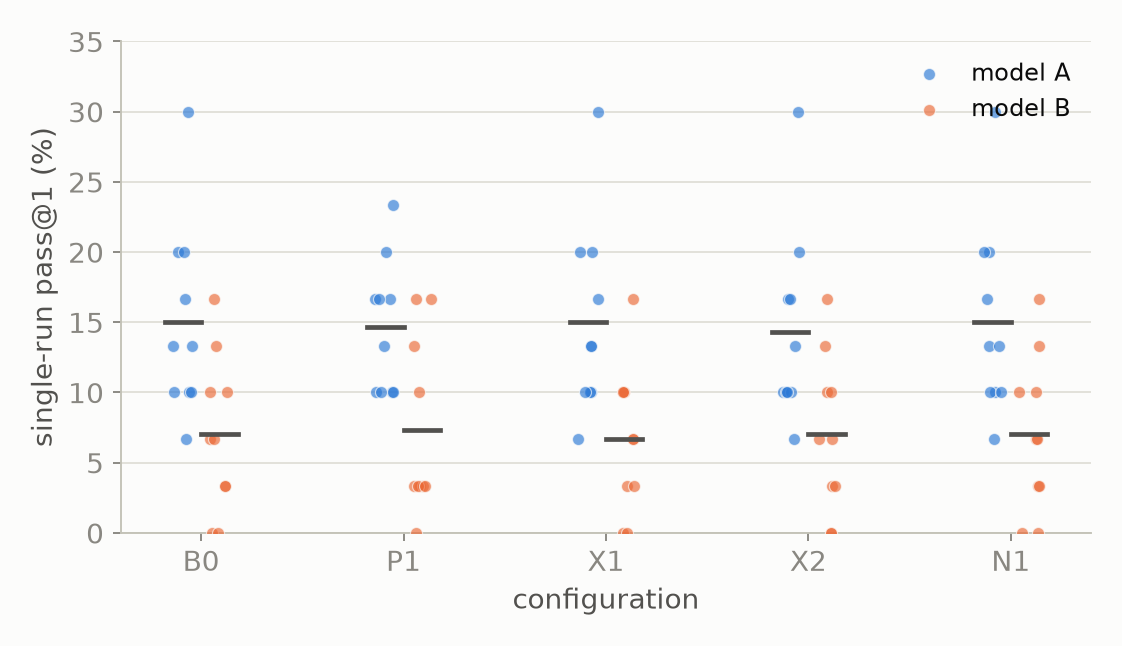
\includegraphics[width=\columnwidth]{rtlsens_pass_at_1.png}
\caption{Single-run pass@1 for both models and each configuration: one dot per sampling seed, with the per-model mean marked. The same model and problems, with only the seed changed, scatter widely (model~A roughly 7--30\%, model~B 0--17\%), while the mean---and hence the configuration---barely moves.}
\label{fig_passat1}
\end{figure}

\noindent \textbf{Factor effects.} Against this noise, every one-factor change is small. Rewording the prompt (P1) moves pass@1 by $-0.3$\,pp; switching the code-extraction rule moves it by $0$\,pp (last-fenced-block, X1) and $-0.7$\,pp (raw module span, X2); automatically renaming the module (N1) moves it by $0$\,pp. The largest of these, X2, is about one-tenth of $\sigma_{\text{seed}}$. Model~B behaves the same way: its largest single-factor effect is 0.3\,pp (X1), again roughly a twentieth of its own $\sigma_{\text{seed}}=5.5$\,pp. Under the decision rule of Section~\ref{sec_m_metrics}---an effect counts only if it exceeds twice $\sigma_{\text{seed}}$ and its confidence interval excludes zero---no factor is material for either model; each is reported as not distinguishable from run-to-run noise. Figure~\ref{fig_factor} places every effect next to the seed-noise line and makes the gap plain.\\

\begin{figure}[htbp]
\centering
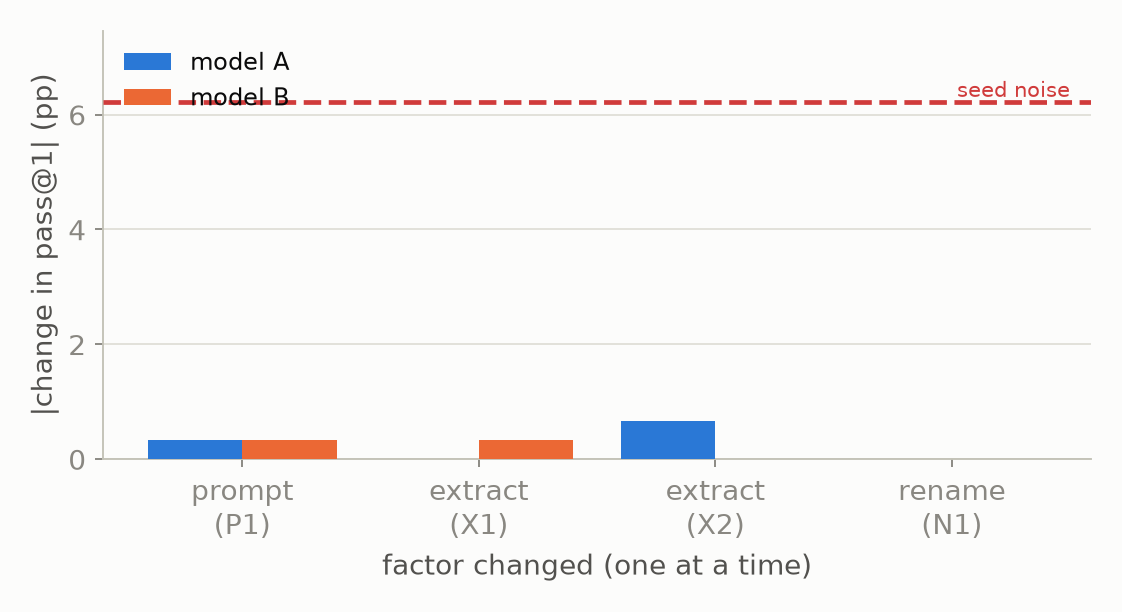
\includegraphics[width=\columnwidth]{rtlsens_factor_effect.png}
\caption{Absolute change in pass@1 from each single-factor edit, for both models, against the run-to-run seed noise $\sigma_{\text{seed}}$ (dashed, averaged over the two models). Every factor sits an order of magnitude below the noise, so none is material at this sample size.}
\label{fig_factor}
\end{figure}

\noindent \textbf{Where the samples fail.} The outcome mix explains why the extraction and naming rules barely matter here: both models almost always emit a fenced code block (no-code rates of about 1\% and 1.5\%), so the extraction choice rarely has anything to disagree about. Most failures are compile errors and functional mismatches rather than missing code, and model~B---the weaker of the two---fails to compile even more often (about 75\% of its samples, against 52\% for model~A), as Fig.~\ref{fig_outcomes} shows. In both cases the bottleneck is writing correct, synthesisable Verilog, not the harness's post-processing, which is exactly why the post-processing factors stay inside the noise.\\

\begin{figure}[htbp]
\centering
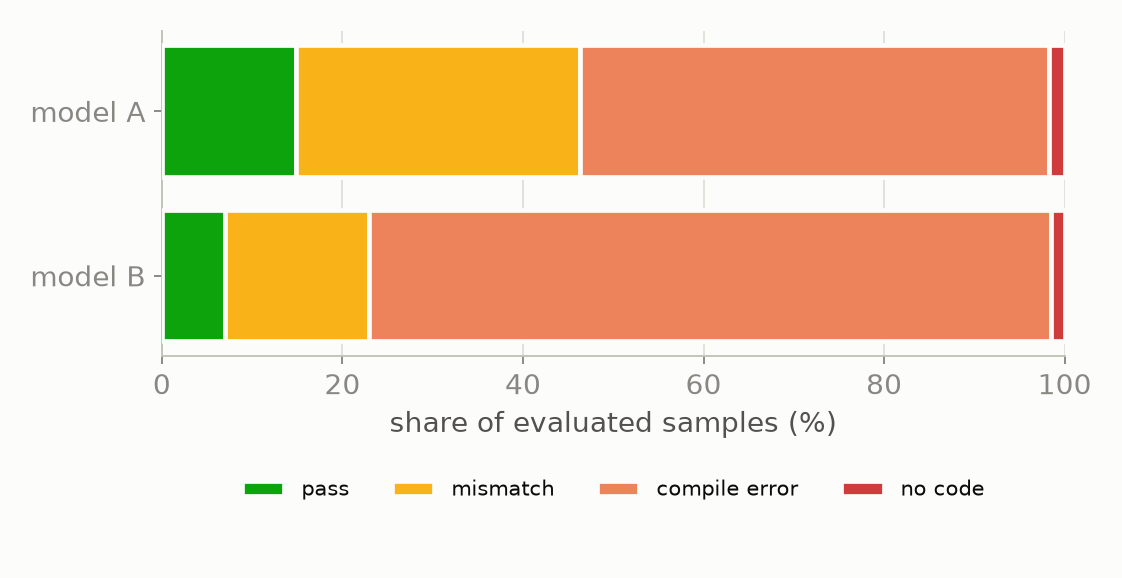
\includegraphics[width=\columnwidth]{rtlsens_outcomes.png}
\caption{Composition of evaluation outcomes for both models across all configurations. A low no-code rate means the extraction rule seldom changes the verdict; most failures are compile errors and mismatches, more so for the weaker model~B.}
\label{fig_outcomes}
\end{figure}

\noindent \textbf{Determinism and gate counts.} At temperature zero both models are fully reproducible: repeated responses are byte-identical and give the same pass/fail outcome on all 30 problems, so seeds can be trusted for the determinism-sensitive parts of the study. The synthesis proxy, by contrast, behaves differently for the two models and gives the one clear example of a tool-side effect that does move. Every passing sample from model~A matches its reference netlist and the three Yosys scripts return identical cell counts, because its passing designs are small combinational blocks whose size is insensitive to the recipe. For model~B, however, the choice of synthesis script changes the cell count by a median of about 64\% between the two end scripts (Y0 versus Y2) across its passing samples---the recipe, not the design, moving the reported size. This is the effect the synthetic-model population-counter test anticipated; the small number of passing designs here makes the exact figure noisy, but the direction is unambiguous and marks the gate-count proxy as the part of the study most in need of the larger subset and of arithmetic-heavy problems.\\

\noindent \textbf{Comparing the two models.} Under the baseline configuration the two models differ in pass@1 by $\Delta_{AB}=8.0$\,pp (15.0\% for model~A against 7.0\% for model~B). Because each model's single-run score already swings by about $\sigma_{\text{seed}}$, a sharper question than ``which scores higher'' is how often a single run would even order them correctly: the reversal probability $\rho$---the chance that one run of the lower-mean model outscores one run of the higher-mean model---is $0.18$. In other words, although model~A's mean is more than double model~B's, roughly one pairing of single runs in six would rank them the wrong way round. The ordering is therefore likely---$\rho$ sits well below the coin-flip value of $0.5$---but not safe to assert from one run of each, which is precisely the single-run-comparison hazard this study set out to quantify.\\

\noindent \textbf{What this adds over a benchmark score.} A conventional RTL benchmark returns a single pass@1 per model \cite{P12_Liu2023,P16_Lu2024}; the VerilogEval revision already notes that this number shifts with prompt phrasing \cite{P15_Pinckney2025}, yet none of them reports how much of the movement is merely seed noise. For the cost of one benchmark run repeated ten times, the pipeline instead returns a characterised measurement: the seed band ($\pm 2\sigma_{\text{seed}}\approx\pm 14$\,pp here), the fraction of movement attributable to each evaluation choice (all $\leq 0.7$\,pp), a temperature-zero determinism rate ($1.0$), and a synthesisability check on every passing sample. Where a benchmark says ``15\%'', this study says ``between roughly 7\% and 30\% depending only on the seed, and essentially unchanged by prompt wording or extraction rule''. The second statement carries more information. The method makes no model look better; it reports how far a model's score can be trusted in the first place, which is the gap current evaluation practice leaves open.\\

\noindent \textbf{Scope and extension.} These numbers come from two small models on half of the subset, so the specific $\sigma_{\text{seed}}$ values and the ordering of factors are a demonstration on real output, not a general law: a stronger model that sometimes omits a code fence could make the extraction rule matter, and arithmetic-heavy designs would move the synthesis proxy further than the single large shift already seen for model~B. The harness, however, is model-agnostic. Pointing it at a 7--8\,billion-parameter model is a one-line change of endpoint, and widening to the full 60-problem subset only multiplies the sample count; neither touches the measurement code. Running the same protocol on larger models and the full subset---the natural next step once a GPU is available---would tighten the confidence intervals and test whether seed noise still dominates once pass rates climb. Only the data would change; the method stays as it is.

\section{Conclusion}\label{sec_conclusion}

Across the studies reviewed here, AI has pushed EDA automation from fixed scripts toward models that predict design metrics, generate RTL, and in a few cases plan whole tool flows---but unevenly across stages, and on benchmarks whose headline numbers prove less stable than they look. This paper reviewed studies covering machine learning, graph neural networks, large language models, and autonomous EDA agents. The proposed five-level automation scale helped compare their capabilities, from scripted workflows to autonomous design flows. The review shows that, although AI has made progress in tasks such as RTL generation, design optimisation, and floorplanning, most existing approaches remain focused on individual stages of the design process. Differences in evaluation methods and the limited use of synthesis and physical design metrics also make direct comparisons difficult.
\\\\
\noindent A key finding is that generating functionally correct RTL is not sufficient for reliable hardware design. AI generated code must also pass synthesis and verification checks before it can be considered useful in practical workflows. The \texttt{rtlsens} framework explores this issue by combining functional simulation with logic synthesis and measuring, one factor at a time, how evaluation choices move the reported pass@1. On a 30-problem subset with two small open models, the run-to-run seed variation (5--7\,pp) dominated every post-processing choice we varied (each $\leq 0.7$\,pp), to the point that a single run of the weaker model beat a single run of the stronger about one time in six despite a two-fold gap in mean accuracy---a direct reminder that a single-run pass@1 is a fragile basis for comparing models. Its evaluation thus highlights both the importance of checking synthesizability and the need to report the seed spread, and not just a point estimate, when quoting RTL-generation accuracy.
\\\\
\noindent Future research should focus on the following areas:
\begin{itemize}
    \item Integrating simulation, synthesis, and verification into closed loop AI workflows to detect and correct errors.
    \item Developing standardised benchmarks that evaluate functional correctness, area, power, and timing across realistic designs.
    \item Improving interoperability, reproducibility, and security through modular architectures, standardised interfaces, controlled execution environments, and detailed logging.
    \item Studying human-AI collaboration and developing privacy preserving models suitable for industrial use.\\
\end{itemize}

\noindent The software-engineering lens contributes one practical rule here: report how much a result moves before reporting the result. When the sampling seed alone swings pass@1 by roughly $\pm 14$\,pp while every evaluation choice we varied moves it by under a point, a single-run score cannot by itself rank two models, and the seed spread belongs in the report beside the mean. Pairing generative models with the deterministic simulation and synthesis checks that catch their errors, and quoting that spread rather than a point estimate, is what moves AI-EDA from isolated experiments toward dependable assistance across the VLSI flow---without removing verification or human oversight from the decisions that need them.

\bibliographystyle{IEEEtran}
\bibliography{ref}

\end{document}